\section{Empirical Experiments} 
In our incentive mechanism, Bayesian inference extracts important and useful information from the collected labels. On the other hand, RIL empowers us with the adaptivity to different kind of workers. In this section, we demonstrate these benefits by empirically testing them one-by-one.

%To demonstrate the benefits of our two core algorithms, Bayesian inference and RL, we empirically test them one-by-one.
%\yitao{To do: better overview for experiments, and need more motivation for 6.1}
%In this section, we firstly test the one-step performance of our incentive mechanism by comparing it with the state-of-the-art incentive mechanism.
%Then, we show the advantages of including the reinforcement algorithm via conducting experiments on three representative worker models, including fully rational, bounded rational and self-learning agents.

\subsection{Performance Analysis of Bayesian Inference}
In this subsection, we focus on our Bayesian inference algorithm by fixing the scaling factor $a^t=1$.
In Figures~\ref{BIM}a-c, we compare the average payments per task for worker $1$ in our incentive mechanism with DG13, the state-of-the-art peer prediction mechanism for binary labels~\cite{dasgupta2013crowdsourced}.
In all these experiments, we set $M=100$, $N=10$, $\mathbb{P}_H=0.8$, $b=0$ and $m_i^t=M(N-1)/N$.
The labels are generated by simulating workers' observation process.
We firstly generate the true label for task $j$ based on the true label distriubtion $(\tau_1, \tau_2)$.
Then, we generate worker $i$'s label for task $j$ based on worker $i$'s PoBC $\mathbb{P}$ and the true label $\mathcal{L}(j)$.
For each point in these figures, we run the experiments for $1000$ rounds and present the means.

In Figure~\ref{BIM}a and b, we show the variation of the payment for worker $1$ with the distribution of true labels and the strategies of other workers, respectively.
More specifically, in Figure~\ref{BIM2}, we let all the other workers report truthfully and exert high efforts ($\mathbb{P}_{i\neq 1}=\mathbb{P}_H$), and meanwhile increase $\tau_1$ from $0.05$ to $0.95$.
In Figure~\ref{BIM3}, we let $\tau_1=0.5$, and increase $\mathbb{P}_{i\neq 1}$ from $0.6$ to $0.95$.
From these two figures, we can find that the payment for worker $1$ in our mechanism almost only depends on worker $1$'s own strategy.
By contrast, the payments in DG13 is severely affected by the distribution of true labels and the strategies of other workers.
In other words, the payment of our mechanism has much better robustness.
Furthermore, in Figure~\ref{BIM4}, we present the standard variance of the payment for worker $1$.
We let $\tau_1=0.5$, $\mathbb{P}_{i\neq 1}=\mathbb{P}_H$ and meanwhile increase $\mathbb{P}_1$ from $0.6$ to $0.95$.
Form the figure, we can find that the payment variance of our mechanism is much smaller than that of DG13.
All in all, compared with traditional peer prediction mechanisms that only compare the labels of two workers, the usage of our variational inference algorithm can improve the robustness and lower the variance of payments, because of its ability of fully exploiting the collected labels.


%Furthermore, in Figure~\ref{BIM1}, we compare our Bayesian inference algorithm with two popular inference algorithms in crowdsourcing, that is, the EM estimator~\cite{raykar2010learning} and the variational inference estimator~\cite{liu2012variational}.
%Here, we set workers' PoBC $\mathbb{P}_i$ to be equal and increase the value of $\mathbb{P}_i$ from $0.5$ to $0.9$.
%The other settings are the same as Figure~\ref{BIM3}.
%From the figure, we can find that, when the quality of labels is very low, the inference bias of the EM and variational inference estimators on the label accuracy can be larger than $0.3$ while the range of the label accuracy is only $[0.5,1.0]$.
%This observation shows that these two estimators become over-optimistic for low-quality labels, which will be disastrous for our RL algorithm.
%Thus, we develop our Bayesian inference algorithm to calibrate the estimates of label accuracy for training our RL algorithm.

\subsection{Empirical Analysis on RIL}
In this subsection, we focus on investigating whether the RIL algorithm proposed in Section \ref{RL} consistently manages to learn a good policy to maximize the data requester's cumulative utility $R=\sum_t r_t$. To demonstrate our algorithm's general applicability, we test it under three distinct worker models, of which each assumes a different rationality level.
For simplicity of experiments, we assume workers always report truthfully,  reducing workers' number of possible strategies on one task from 4 to 2 (i.e choosing only between high and low efforts). 
We provide a formal description about the three models as follows
\begin{itemize}[topsep=0pt, partopsep=0pt]
\item {\bf Rational} workers alway act to maximize their own utilities. Since our incentive mechanism theoretically ensures that exerting high effort % and reporting truthfully 
is the utility-maximizing strategy for all workers (proved in Section~\ref{analysis}), it is safe to assume workers always do so as long as the payment is high enough to cover the cost.
\item {\bf Quantal Response (QR)} workers \citep{mckelvey1995quantal} exert high efforts with the probability 
$$
\textsf{eft}_i^t= \frac{\exp(\lambda\cdot  u_{iH}^t)}{\exp(\lambda \cdot u_{iH}^t) + \exp (\lambda \cdot u_{iL}^t)}
$$
where $u_{iH}^t$ and $u_{iL}^t$ denote worker $i$'s expected utility after exerting high or low efforts respectively at time $t$. $\lambda$ describe workers' rationality level and we set $\lambda =3$.

\item {\bf Multiplicative Weight Update (MWU)} workers \citep{chastain2014algorithms} update their probabilities of exerting high efforts at every time step $t$ after receiving the payment as the following equation
\begin{align*}
\textsf{eft}_i^{t+1} = \frac{\textsf{eft}_i^t(1+\bar{u}_{\cdot H})}{\textsf{eft}_i^t(\bar{u}_{\cdot H} - \bar{u}_{\cdot L}) + \bar{u}_{\cdot L} + 1}
\end{align*}
where $\bar{u}_{\cdot H}$ and $\bar{u}_{\cdot L}$ denote the average utilities received if exerting high efforts or low efforts at time $t$ respectively. We initialize $\textsf{eft}_i^0$ as $0.2$ in our experiments.
\end{itemize}


In all these experiments, we set $M=100$, $N=10$, $\mathbb{P}_H=0.8$, $b=0$, $c_H=0.02$, the available value set of the scaling factor $\mathcal{A}=\{0.1,1.0,5.0,10\}$, the exploration rate $\epsilon = 0.2$ for RIL, $F(A)=A^{10}$ and $\eta=0.1$ for the utility function (Eqn.\ref{equation:utility}).
Traditional peer prediction mechanisms are often applied by manually setting a value for the scaling factor.
Since we have shown the advantages of using Bayesian inference in Section 6.1, we use our payment rule with the manually adjusted scaling factor as the benchmark. 
In this case, how the tasks are assigned does not affect the comparision and thus we let every worker get assigned the whole task set (i.e. $\forall i, m_i^t = M$).
Besides, in each episode of Algorithm~\ref{RAC}, we set the number of steps as $28$.
%Besides, for simplicity of experiments, we assume workers always report truthfully. This reduces the number of a worker's possible internal states from $4$ to $2$.
%Furthermore, to reduce the influence of outliers, we report the average over 5  trials in all the figures.

%make several assumptions. First, we assume workers always report truthfully. This reduces the number of a worker's possible internal states from 4 to 2. Second, we assume at each time $t$, every worker gets assigned the whole task set (i.e. $\forall i, m_i^t = M$). \yitao{why those assumptions make sense} Furthermore, to reduce the influence of outliers, we report the average over 5  trials. In order to show our method applies to the most general settings, we set up our experiments using 3 different existing worker models:
%
%effectively cooperate with other components, and more importantly, whether it manages to learn a good policy under this inherently noisy environment to maximize the data requester's cumulative utility $\sum_t r^t$. Furthermore, we wish this subsection would provide deeper insights for readers into how reinforcement learning would be helpful in constructing a strong incentive mechanism.
%
%For simplicity of experiments, we make several assumptions. First, we assume workers always report truthfully. This reduces the number of a worker's possible internal states from 4 to 2. Second, we assume at each time $t$, every worker gets assigned the whole task set (i.e. $\forall i, m_i^t = M$). \yitao{why those assumptions make sense} 
 

%In order to show our method applies to the most general settings, we set up our experiments using 3 different existing worker models:
%\begin{itemize}
%\item {\bf Rational}: A rational worker alway acts to maximize his or her own utlity. Since our mechanism theoretically ensures that exerting high effort and reporting truthfully is the utility maximizing strategy for all workers, it is safe to assume workers always do so as long as the payment is high enough to cover the cost.
%\item {\bf Quantal Response} \citep{mckelvey1995quantal}: A quantal response (QR) worker exerts high efforts with the probability 
%$$
%\textsf{eft}_i^t= \frac{\exp(\lambda\cdot  u_{iH}^t)}{\exp(\lambda \cdot u_{iH}^t) + \exp (\lambda \cdot u_{iL}^t)}
%$$
%where $u_{iH}^t$ and $u_{iL}^t$ denote worker $i$'s expected utility after exerting high or low efforts respectively at time $t$. $\lambda$ describe workers' rationality level and we set $\lambda =3$ in our experiments.
%
%\item {\bf MWU} \citep{chastain2014algorithms}: A multiplicative weight update (MWU) worker updates his/her probability of exerting high efforts at every time step $t$ after receiving the payment as the following
%\begin{align*}
%\textsf{eft}_i^{t+1} = \frac{\textsf{eft}_i^t(1+\bar{u}_{\cdot H})}{\textsf{eft}(\bar{u}_{\cdot H} - \bar{u}_{\cdot L}) + \bar{u}_{\cdot L} + 1}
%\end{align*}
%where $\bar{u}_{\cdot H}$ and $\bar{u}_{\cdot L}$ denote the average utility if exerting high efforts or low efforts respectively.
%\end{itemize}
%Besides, we set $\mathbb{P}_H = 0.9$, $\mathbb{P}_L = 0.5$ and $c_{H} =0.02$.

Our first set of experiments focuses on the estimation bias of the the data requester's cumulative utility $R$.
Since the data requester's utility is used as the reward signal for our RL algorithm, it would not be a surprise that the reliability of the estimation plays a crucial role in determining the well-being of the whole mechanism. As Figure~\ref{figure:rewardError} shows, the estimated value's deviation from the real one will become very small after some episodes of learning, regardless of which worker model the experiments run on.
This means the learned reward signal provides a good guidance for our RL algorithm.
The next set of experiments is about how quickly our RL algorithm learns. As Figure~\ref{figure:learningCurve} shows, for all the three worker models, our RL algorithm manages to pick up a policy to maximize the cumulative utility of the data requester in less than 100 episodes. 
This observation shows the consistently good performance on different worker models.

%Besides, from the figure, we can find that our RL algorithm converges the fastest on the rational workers. This is because the optimal policy for the rational workers is to let $a_t\equiv=0.1$ so that the payment will be minimized.
%Compared with the stochastic policy on the other two kinds of workers, this policy is easy to learn and thus our RL algorithm coverges the fastest.

%we conduct focuses on the accuracy of the estimation of the data requester's cumulative utility $R$. Since it is used as the reward signal for our RL algorithm, it would not be a surprise that the reliability of the estimation plays a crucial role in determining the well-being of the whole mechanism. As Figure~\ref{figure:rewardError} shows, the estimated value's deviation from the real one is small, regardless of which worker model the experiments run on. Besides, we can observe a large deviation at the begining stage of the training on the QR workers. This is because the small scaling factor at the begining stage causes the difference between $u^t_{iH}$ and $u^t_{iL}$ to be very small, which will lead to low-quality labels. Even though our Bayesian inference algorithm has significantly reduce the bias on low-quality labels, the cumulative errors is still very large, which shows the necessity of our inference algorithm.
%Furthermore, the deviations on the rational and QR workers both will converge to a very small value while the deviation on the MWU worker will stay at relatively large values.
%This is because the first two kinds of workers responds to the incentives in a fixed way. Once we find the optimal scaling factor, we can always use this value and get high-qualtiy labels.
%By contrast, MWU workers must have a process to learn the benefits of exerting high efforts. In this stage, the label quality will be very low, leading to a quite large deviation.


\begin{figure}[!t]
   \setlength{\abovecaptionskip}{0mm}
    \centering
    \begin{subfigure}[t]{0.24\textwidth}
        \centering
        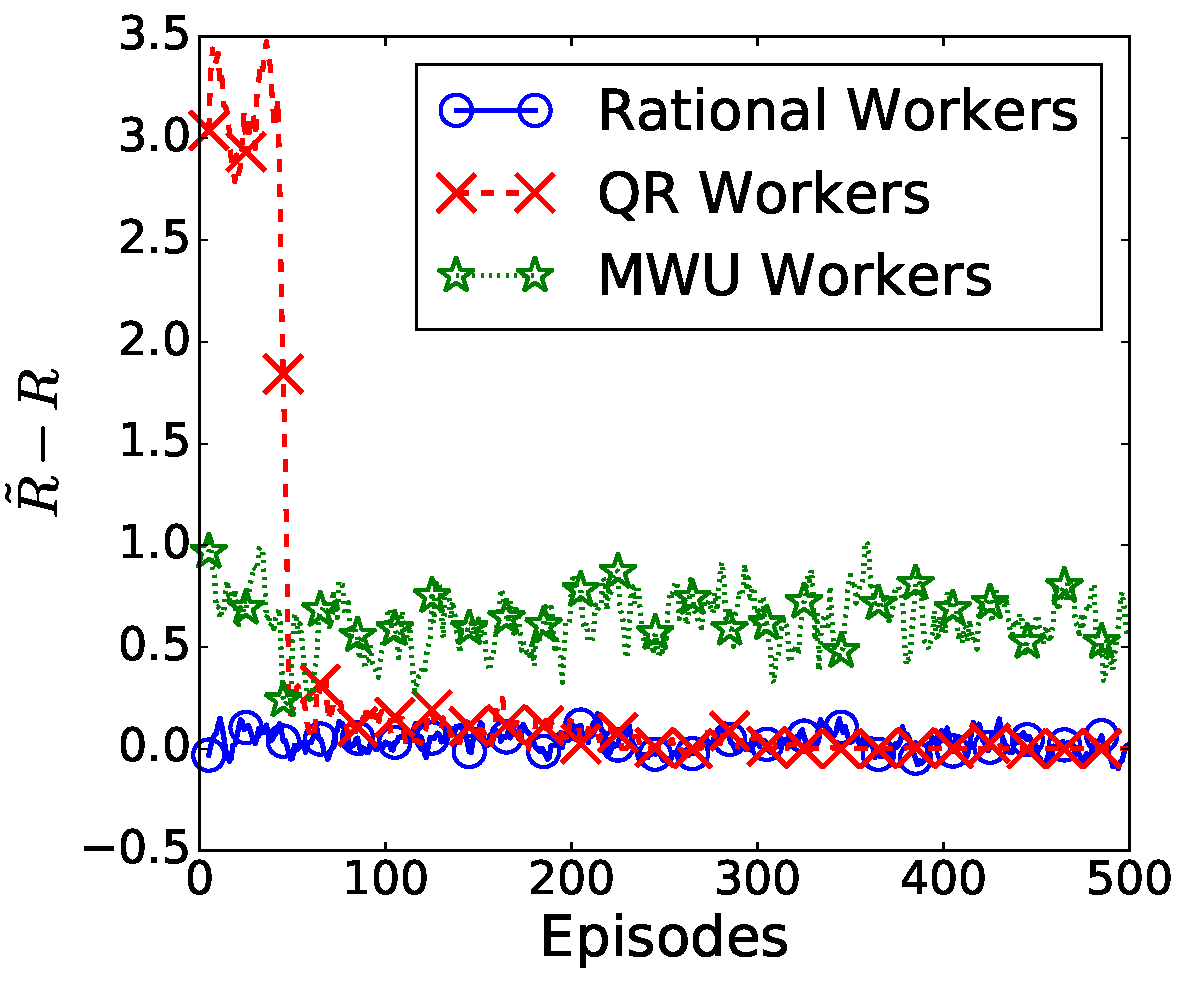
\includegraphics[width=\textwidth]{image/RIL1}%rewardError
		\vspace{-1mm}
        \caption{\label{figure:rewardError}}
    \end{subfigure}%
~
    \begin{subfigure}[t]{0.23\textwidth}
        \centering
        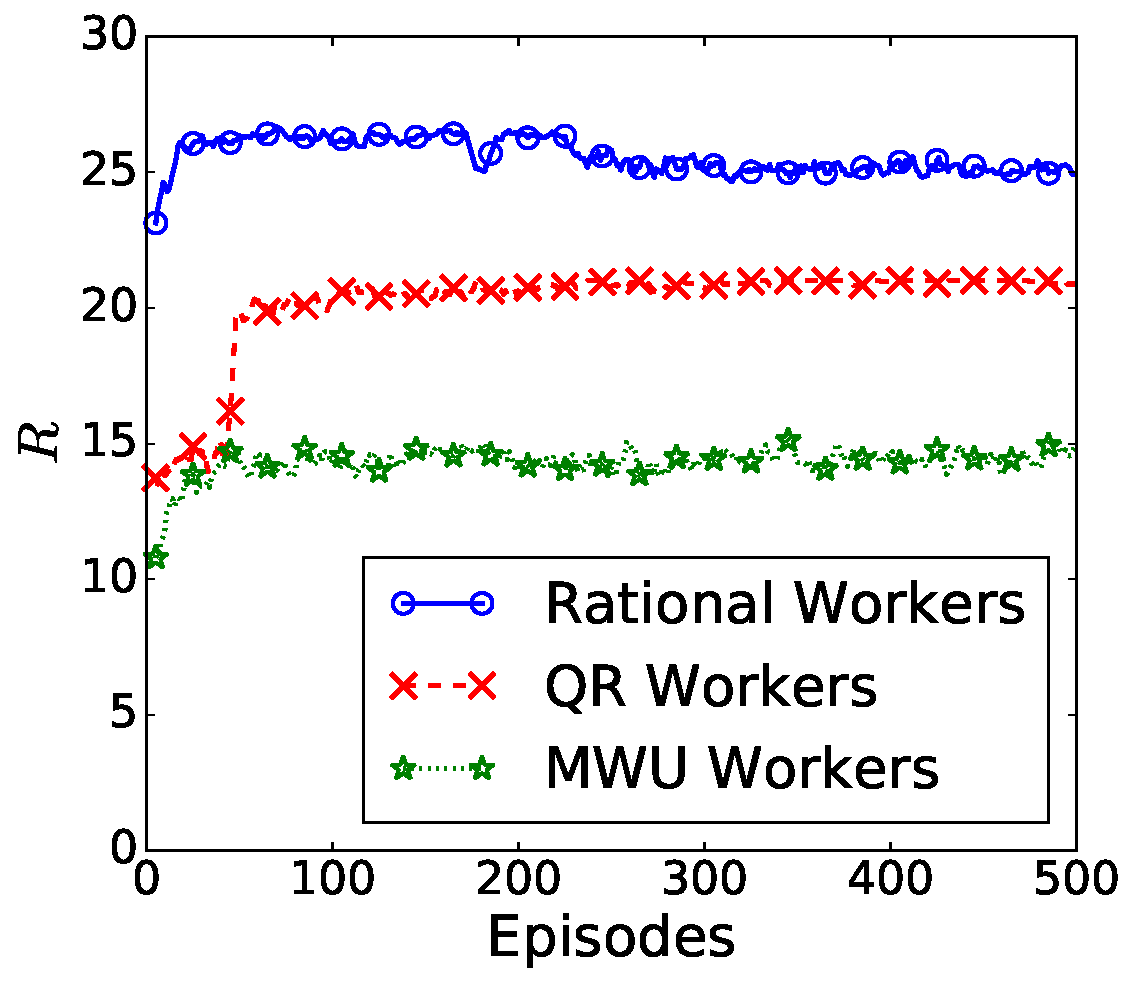
\includegraphics[width=\textwidth]{image/RIL2}%learningCurve
		\vspace{-1mm}
        \caption{\label{figure:learningCurve}}
    \end{subfigure}
    \caption{\label{figure:learning}Empirical analysis on our RL algorithm (a) the gap between the estimation of the data requester's cumulative rewards and the real one, smoothed over 5 episodes (b) the learning curve of our mechanism smoothed over 5 episode}
	\vspace{-2mm}
\end{figure}
%\begin{figure}[t]
%\centering
%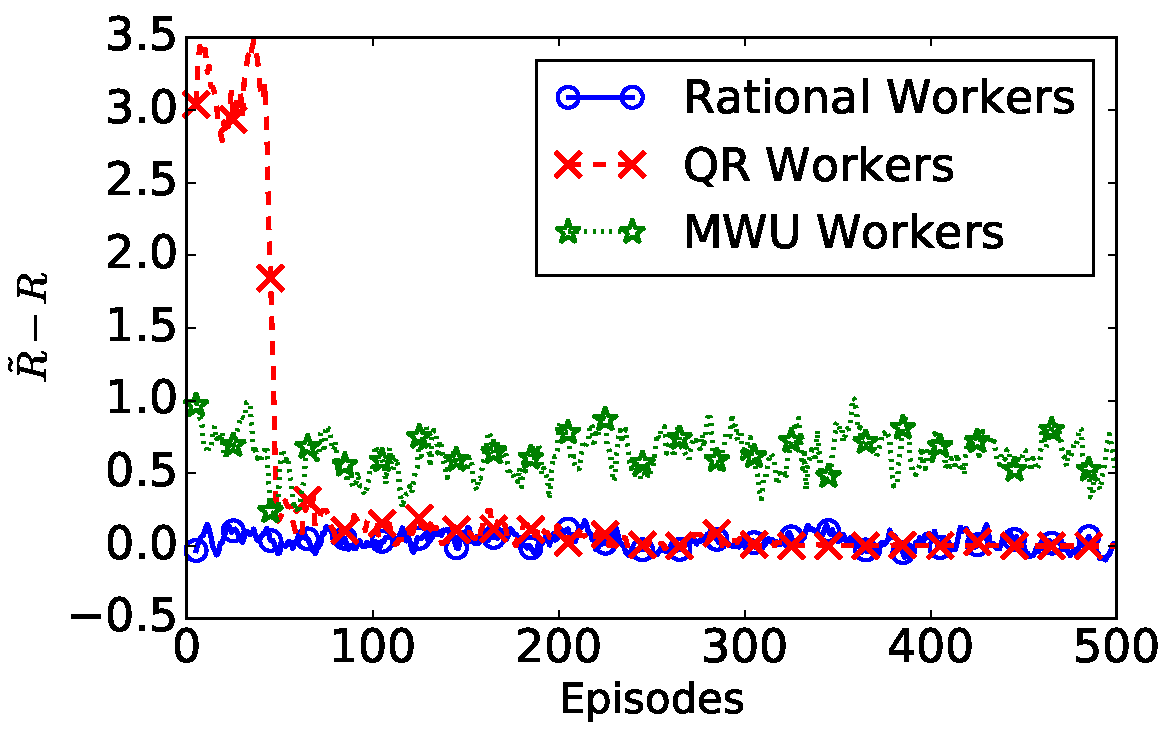
\includegraphics[scale=0.4]{image/rewardError}
%\vspace{-2mm}
%\caption{The gap between the estimation of the data requester's cumulative reward and the real one, smoothed over 5 episodes.}
%\label{figure:rewardError}
%\end{figure}
%

%
%\begin{figure}[t]
%\centering
%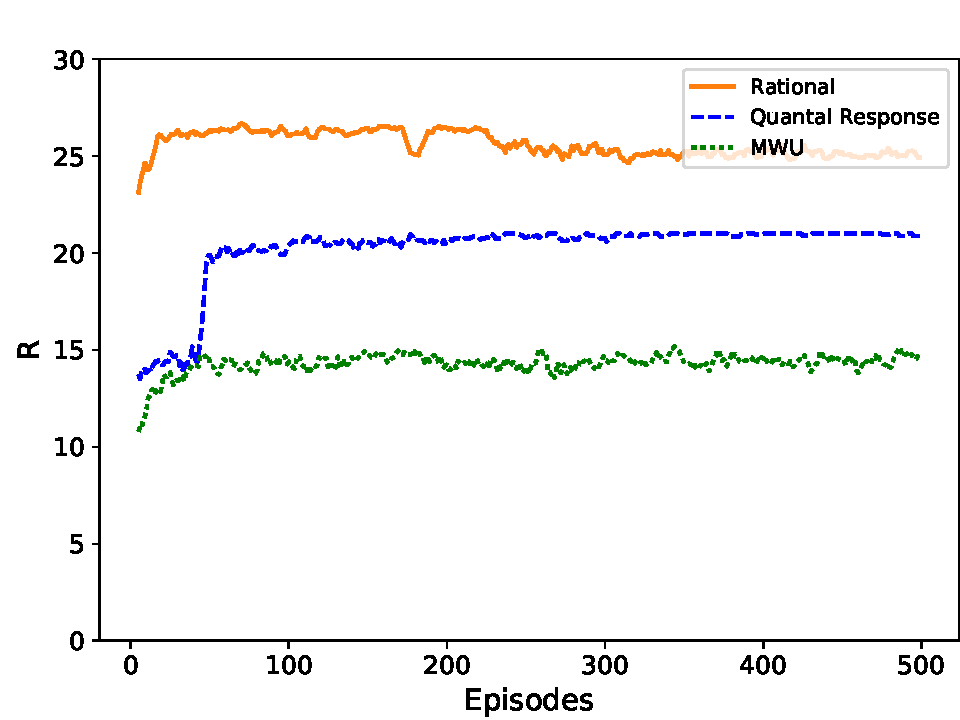
\includegraphics[scale=0.4]{image/learningCurve}
%\vspace{-2mm}
%\caption{The learning curve of our mechanism smoothed over 5 episodes.}
%\label{figure:learningCurve}
%\end{figure}

Lastly, we take the learned policy of our RL algorithm and compares it with two benchmarking policies in Table~\ref{table:performance}. The first policy, Fixed Optimal, sets a fixed value for the scaling factor, which is commonly adopted by existing mechanisms. Here, to conduct comparison, we try all possible values and output the highest cumulative rewards in Table~\ref{table:performance}. The second policy, Adaptive Optimal, changes the scaling factor every $4$ steps and find highest cumulative rewards via traversing all $4^7=16384$ possible value combinations of the scaling factor. This policy is impossible in practice but very close to the real optimal.
From Table~1, we can find that the three policies have shown similar performance for rational and QR workers.
This is because these two kinds of workers has a fixed pattern in response to incentives and thus the optimal policy should be to set a fixed value for the scaling factor.
By contrast, MWU workers needs to learn their utility-maximizing strategies gradually, and the learning process is affected by the incentives.
For this model, compared with Fixed Optimal, our RL algorithm increases the cumulative reward from $11.7$ to $15.6$, which is a significant improvement considering the unreachable real optimal is only around $18.5$. To summarize, our RL algorithm can consistently improve the cumulative utility of the data requester over different worker models.

\begin{table}
   %\setlength{\belowcaptionskip}{2mm}
\caption{
\label{table:performance}Performance comparison on three worker models.}
\centering
{\scriptsize
\begin{sc}
\begin{tabular}{ l | l | l | l }
\hline
Method & Rational & QR & MWU \\ \hline \hline
Fixed Optimal & 27.584 (.253) & 21.004 (.012) & 11.723 (.514) \\
Adaptive Optimal & 27.618 (.109) & 21.017 (.004) & 18.475 (.382) \\
RIL & 27.184 (.336) & 21.016 (.018) & 15.726 (.416)\\
\hline
\end{tabular}
\end{sc}
}
\vskip -0.1in
\end{table}
%We plot the deviation of the estimated value from the real one in Figure~\ref{figure:rewardError}




%In the literature of crowdsourcing, the Dawid-Skene estimator is the most popular method used to infer the true labels~\cite{dawid1979maximum,raykar2010learning}.
%The variational inference estimator, which has the similar Bayesian model to our inference algorithm, is also widely-adopted in the existing studies of crowdsourcing~\cite{liu2012variational,chen2015statistical}.
%To compare different estimators, we set $M=100$ and $N=10$ in Figure~\ref{BIM1}. Also, we let the score of all workers be equal, namely $p_1= \ldots=p_N$, and increase the value of $p_i$ from $0.5$ to $0.9$. Meanwhile, we set the true label distribution as the uniform distribution, namely $\tau_1=\tau_2=0.5$. For a given $p_i$, we firstly generate the true labels and then the labels of all workers both by the Bernoulli distribution. For each value of $p_i$, we run the experiments for $1000$ rounds. To show the bias of inference, we calculate the average value differences between the posterior expected accuracy $\mathbb{E}A$ and the real accuracy $A$. From the figure, we can find that, when workers can provide not-so-bad labels ($p_i>0.75$), both the two above estimators and our inference algorithm have very small bias, which agrees with the good performance of these estimators in the literature~\cite{raykar2010learning,liu2012variational}. However, if workers can only provide low-quality labels, the bias of the Dawid-Skene and variational inference estimators will become unacceptable, because the difference can be larger than $0.3$ while both $\mathbb{E}A$ and $A$ belong to $[0.5,1.0]$. In this case, we cannot use $\mathbb{E}A$ to calculate the utility of the data requester as Equation~\ref{utility}. By contrast, the bias of our Bayesian inference algorithm is much smaller, which is the foundation of our reinforcement incentive mechanism.
%
%
%In Figures~\ref{BIM}b-d, we focus on $r_1$, namely, the per-task-reward received by worker $1$. Here, DG13~\cite{dasgupta2013crowdsourced,liu2017sequential}, which is the state-of-the-art incentive mechanism for binary labels, is employed as the benchmark.
%DG13 decides the reward for a worker by comparing his labels with the labels provided by another randomly selected worker.
%By elaborately designing the reward rules, it can also ensure reporting truthfully and exert high efforts to be a Nash equilibrium for all workers.
%In all these experiments, we set $p_H=0.8$, $p_L=0.5$, and keep the other settings the same as those in Figure~\ref{BIM1}.
%
%In Figure~\ref{BIM2}, we let $p_{-1}=p_H$, where the subscript $-1$ denotes all the workers except for worker $1$.
%We change the distribution of true labels by increasing $\tau_1$ from $0.05$ to $0.95$ and compare the average values of $r_1$ corresponding to the different strategies of worker $1$.
%In Figure~\ref{BIM3}, we fix the distribution of true labels to be the uniform distribution, namely, $\tau_1=\tau_2=0.5$, and increase $p_{-1}$ from $0.6$ to $0.95$.
%From these two figures, we can find that the rewards provided by our mechanism are almost not affected by the variation of the distribution of true labels and the strategies of the other workers.
%This observation reveals that $\mathbb{E}\tilde{p}_1$ converges to $p_1$ in most cases.
%The only exception is $p_{-1}<0.7$ in Figure~\ref{BIM3} where the low-quality labels will lead to a remarkable bias of inference.
%Even in this case, worker $1$ can only get the maximal reward when $p_1=p_H$, which shows the attracting ability of our mechanism to induce truthful reports and high efforts.
%By contrast, $r_1$ in DG13 is severely affected by the distribution of true labels and the strategies of other workers.
%For example, in Figure~\ref{BIM3}, if the other workers lower their efforts, the reward received by worker $1$ will also decrease, although worker $1$ never changes his strategies.
%Thereby, for worker $1$, our Bayesian incentive mechanism is much fairer than DG13.
%
%In Figure~\ref{BIM4}, we set $\tau_1=\tau_2=0.5$ and $p_{-1}=p_H$. We change worker $1$'s strategies by increasing $p_1$ from $0.6$ to $0.95$. Under these settings, the average values of $r_1$ corresponding to our mechanism and DG13 both can reflect the variation of $p_1$ very well. Thus, we focus on the standard variance comparison of $r_i$ in Figure~\ref{BIM4}.
%If the variance is very large, the reward received by worker $1$ when $p_1=p_H$ may become lower than the reward when $p_1<p_H$.
%If this case happens, it will significantly discourage worker $1$.
%For example, in Figure~\ref{BIM2}, when $\tau_1=0.05$, for DG13, the difference between $r_1(p_1=p_H)$ and $r_1(p_1=0.5)$ is around $0.06$.
%On the other hand, from Figure~\ref{BIM4}, the standard variance of $r_1$ is around $0.052$, which means there is a quite high probability for $r_1(p_1=p_H)<r_1(p_1=0.5)$.
%From Figure~\ref{BIM4}, we can find that our Bayesian incentive mechanism has a lower variance than DG13.
%If we take the fairness of our mechanism into consideration, we can conclude that our mechanism is more stable than DG13 in inducing truthful reports and high efforts from workers.


%\begin{equation}
%P(L(j)=1)=\tau_1{\prod}_{k\neq i}p_H^{\delta_{kj1}}(1-p_H)^{\delta_{kj2}}
%\end{equation}
%where $\lambda_0=\log(\tau_1/\tau_2)$ and $\lambda_i=\log(p_i/\bar{p}_i)$. For worker $i$, we assume that all other workers report truthfully and exert high efforts. Suppose the real true label is $1$. In order to ensure $\mathbb{E}[m/M]$ to approach $0$, the probability ratio in Equation~\ref{Ratio} must be positive with almost $1.0$ probability. Thus, we can directly discard the absolute operation in Equation~\ref{vot} and calculate the expected value of task $j$ as
%\begin{equation}
%\mathbb{E}_1v(j)\approx \lambda_0+(N-1)(2p_H-1)\lambda_H+(2p_i-1)\lambda_i.
%\end{equation}
%Similarly, if the real true label is $2$, then
%\begin{equation}
%\mathbb{E}_2v(j)\approx -\lambda_0+(N-1)(2p_H-1)\lambda_H+(2p_i-1)\lambda_i.
%\end{equation}
%Thus, the average task value $v$ satisfies
%\begin{equation}
%\begin{split}
%&\mathbb{E}v = \tau_1 \mathbb{E}_1v(j) + \tau_2\mathbb{E}_2v(j)\\
%&=(2\tau_1-1)\lambda_0+(N-1)(2p_H-1)\lambda_H+(2p_i-1)\lambda_i.
%\end{split}
%\end{equation}
%
%Suppose the true label is $1$.
%\begin{equation}
%x= \log\frac{P(L=1)}{P(L=2)}=g+\sum_{i=1}^{N}f(x_i,y_i,w_i,z_i)
%\end{equation}
%\noindent where $g=g_1-g_2$, and 
%\begin{equation*}
%g_1=\log(s_1+t_2+1)\;,\;g_2=\log(s_2+t_1+1).
%\end{equation*}
%Omitting the subscript in $f$, we can have $f=f_1-f_2$ with probability $p$ and $f=f_2-f_1$ with probability $1-p$. Here,
%\begin{equation*}
%f_1=\log(x+z+2)\;,\;f_2=\log(w+y+1).
%\end{equation*}
%Thus, we can have
%\begin{equation}
%\mathbb{E}g = \mathbb{E}g_1-\mathbb{E}g_2 \;,\;
%\mathbb{E}f = (2p-1)(\mathbb{E}f_1-\mathbb{E}f_2).
%\end{equation}
%From the previous proof, we know that $P(m)$ is very small when $m>>1$. Thus, we mainly focus on the region where $m$ is relatively small. For a given small $m$,
%\begin{equation}
%\mathbb{E}_{s_1, t_2}g_1\approx \mathbb{E}_{t_2}\log(np+t_2+1)
%\end{equation}
%\begin{equation}
%\log(np+t_2+1) = \log(np+1)+\sum_{i=1}^{\infty}(-1)^{i-1}q^i
%\end{equation}
%\begin{equation}
%q = \frac{t_2}{np+1}\Rightarrow 0\leq q^{i} \leq c^{i}\cdot \left(\frac{m}{M}\right)^i\leq c^{i}\frac{m}{M}
%\end{equation}
%Then,
%\begin{equation}
%\mathbb{E}g_1 \approx \mathbb{E}_{m}\log(1+Mp-mp)
%\end{equation}
%\begin{equation}
%\log(1+Mp-mp)\approx\log(1+Mp)+\sum_{i=1}^{\infty}(-1)^{i}\left(\frac{m}{M}\right)^i
%\end{equation}
%Using the similar way of approximation for the computation of $\mathbb{E}g_2$, $\mathbb{E}f_1$ and $\mathbb{E}f_2$, we can have
%\begin{equation}
%\begin{split}
%\mathbb{E}g_1\approx \log(Mp)\;,\;\mathbb{E}g_2\approx \log(M(1-p))\\
%\mathbb{E}f_1\approx \log(Mp)\;,\;\mathbb{E}f_2\approx \log(M(1-p))
%\end{split}
%\end{equation}
%Thus, if all workers exert high efforts and report truthfully,
%\begin{equation}
%    \mathbb{E}x \approx \log\lambda_0 + {\sum}_{i=1}^{N}\log\lambda_{i,H}
%\end{equation}
%If the true label is $2$, then
%\begin{equation}
%    \mathbb{E}x \approx \log\lambda_0 - {\sum}_{i=1}^{N}\log\lambda_{i,H}
%\end{equation}
%Thereby,
%\begin{equation}
%    \mathbb{E}|x|\approx (2p_0-1)\log\lambda_0+ {\sum}_{i=1}^{N}\log\lambda_{i,H}
%\end{equation}
%When, for example, worker $1$ deviate from the desired equilibrium strategy, the non-equilibrium state correspond to
%\begin{equation}
%    \mathbb{E}|x'|\approx (2p_0-1)\log\lambda_0+ \log\lambda_{1}+{\sum}_{i=2}^{N}\log\lambda_{i,H}
%\end{equation}
%The minimal value of $\mathbb{E}|x'|$ is reached when worker $1$ exert high efforts and report falsely, namely $\log\lambda_{i}=-\log\lambda_{i,H}$.
%Thus, the maximal reward increment brought by worker $1$'s strategy switch is
%\begin{equation}
%    V_1 = F(\mathbb{E}x)-F(\mathbb{E}x') \approx 2\log\lambda_{1,H}\cdot \left.\frac{\mathrm{d}F}{\mathrm{d}x}\right|_{x=x_H}
%\end{equation}
%Since $p_0$ is difficult to estimate, we define the upper bound of the value increment as
%\begin{equation}
%    V = 2\max_{i}\log\lambda_{i,H} \cdot  \max_{x\in [x_H, \infty)}\frac{\mathrm{d}F}{\mathrm{d}x} 
%\end{equation}
%where $x_H= \log\lambda_0 + {\sum}_{i=1}^{N}\log\lambda_{i,H}$.
%Considering the discounted reward calculation in reinforcement learning, we can know the maximum value difference can be created by the manipulation of any worker is $(1-\rho)^{-1}V$. Meanwhile, if the reinforcement part increases the scaling factor by $\delta$ to obtain the reward increment, we need to pay more than $\sum_{i=1}^{N}M\delta (p_{i,H}-0.5)$. Thus, if we want to prevent the reinforcement learning module from the adversarial manipulation, the minimal gap $\delta$ between to two available scaling factors should satisfy
%\begin{equation}
%    \sum_{i=1}^{N}M\delta (p_{i,H}-0.5) > V.
%\end{equation}